\section{\sys Design}\label{sec:design}
\begin{figure*}[t]
% \centering
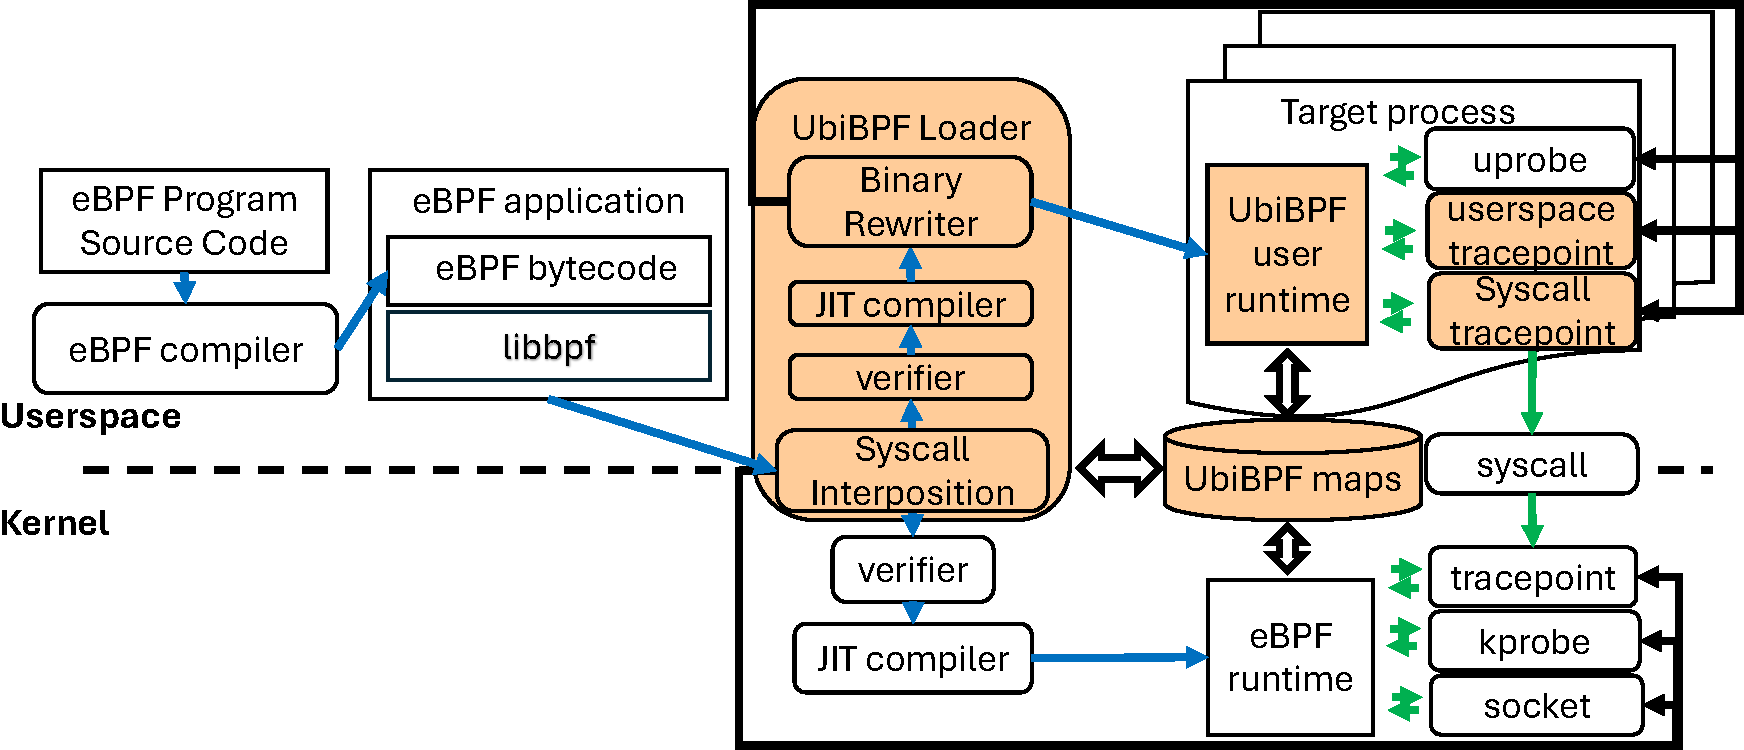
\includegraphics[width=.6\textwidth]{img/bpftime-diagram-cropped.pdf}
\caption{\sys{} Design.  White components are the same between \sys{} and eBPF; orange components are new to \sys{}. Arrow colors are consistent with \cref{fig:eBPF-design}. }\label{fig:bpftime-design}
\end{figure*}

\sys{} is a comprehensive, dynamic, safe, and efficient extension framework built using our two guiding principles: compatibility with the eBPF ecosystem and userspace extension execution without kernel involvement.  The system solves the three main challenges (\cref{sec:challenges}) that arise when following these principles: \sys{} solves the challenge of providing an eBPF-compatible runtime through the \sys{} Loader, a layer of interposition between the eBPF application and kernel that is feature-compliant with ebpf; the \sys{} maps, a new implementation of eBPF maps that allows userspace extensions and eBPF applications to interact without kernel involvement; and a collection of userspace eBPF helper functions.  \sys{} solves the challenge of trap-free extensions by adopting techniques from binary rewriting~\cite{Dinesh20, Chamith17, WilliamsKing20, fridagum}.  Finally, \sys{} ensures safety by using a userspace eBPF bytecode verifier~\cite{Gershuni19} to prevent a buggy extension from harming an application, and uses hardware memory protection~\cite{Vahldiek19, xie2022cetis} to prevent a buggy or subverted applications from circumventing an extension.  \Cref{fig:bpftime-design} shows the design.

\paragraph{Usage} \sys{}'s usage mirrors that of eBPF: a user writes an event-based eBPF program.  \sys{} provides a new type of hook point for the user, a \texttt{userspace} \texttt{tracepoint}, which an application developer can add to their code to support custom hook points, similar to \texttt{tracepoint}s in the kernel.  The user then compiles their program using an eBPF compiler.  At runtime, the user executes their eBPF application.  The eBPF application uses eBPF-related system calls, which the \sys{} loader interposes upon.  The loader verifies that the extensions are safe to execute, initializes data in the \sys{} maps for the application, initializes the \sys{} user and eBPF runtimes, and attach extensions to their hook points.  The \sys{} user runtime uses hardware isolation to ensure that extensions are safe from subverted applications.  During execution, the \sys{} user and eBPF runtimes execute extensions each time the userspace and kernel reach hook points, respectively.

The rest of this section describes \sys{}'s key components: the \sys{} loader (\cref{sec:design:loader}), the \sys{} user runtime (\cref{sec:design:UVM}), and the \sys{} maps (\cref{sec:design:maps}). 

\subsection{\sys Loader}\label{sec:design:loader}
The \sys{} loader prepares eBPF extensions in an eBPF application for execution.  The loader is a layer of interposition between an eBPF application and the kernel; it exposes the  eBPF-related system calls interface from the eBPF ecosystem, allowing \sys{} to support existing eBPF application frameworks (e.g., bcc and libbpf). 

The \sys{} loader first separates an eBPF application's extensions into userspace extensions and kernel extensions.  The system uses the conventional eBPF ecosystem's design to load kernel extensions; see \cref{sec:challenges:eBPF-background} for details. 

To load userspace extensions, the system first ensures that they are safe using an eBPF userspace verifier~\cite{Gershuni19}.  Similar to the in-kernel verifier (\cref{sec:challenges:eBPF-background}), the userspace verifier ensures that an extension is memory and type safe, guaranteed to terminate, and will not execute a hardware exception.  \sys{} adds two things to support its userspace eBPF bytecode verification.  First, it provides verification support for its userspace helper functions, including for map access (\cref{sec:design:UVM}).  Second, \sys{} parses DWARF debugging information to produce BTF information for the target application.  Once verified, extensions pass through a userspace JIT compiler, which compiles them into native code. The JIT compiler passes the compiled extensions to a binary rewriter. 

The binary rewriter uses \texttt{ptrace} to pause the target application and load the \sys{} user runtime (\cref{sec:design:UVM}) into it; this approach ensures dynamism.   The rewriter instruments the program's instructions to ensure that eBPF functions are invoked when the program reaches their associated \texttt{uprobe}, \texttt{uretprobe}, \texttt{syscall} \texttt{tracepoint}, or \texttt{userspace} \texttt{tracepoint}.  The rewriter supports \texttt{uprobe}s, \texttt{uretprobe}s, and \texttt{userspace tracepoint}s using a standard instruction trampoline: it replaces the instructions that were originally at the hook point with a \texttt{call} into a preamble for the point's associated eBPF function and places the overwritten instructions at the end of its preamble.  Supporting extensions to \texttt{syscall tracepoint}s is more complex.  Whereas other extensions should be invoked when a program reaches a specific userspace instruction, a extension to a \texttt{syscall tracepoint} should be invoked anytime the application executes a system call instruction (\ie \texttt{sysenter}), which are scattered throughout an application and its shared libraries.  To support this, the runtime iterates through all of the instructions in the application and places a trampoline on all system call instructions.  Since \texttt{sysenter} is smaller than a trampoline, the system uses zpoline~\cite{yasukata2023zpoline}, which uses the zero page to accommodate two-byte call instructions.

In addition to loading the eBPF extensions into the target application, the \sys{} loader also initializes the \sys{} maps required for the eBPF application. This process requires handling symbol relocations so that \sys{} can support multiple simultaneous eBPF applications.

% The \sys{} Daemon's eBPF bytecode verifier iterates through the instructions of the user-provided eBPF bytecode.  It ensures memory safety by checking that the type and memory offset of each memory dereference is correct by using the BPF Type Format (BTF).  The BTF includes low-level information about all structs referenced in the program, \eg their field offsets.  The verifier ensures termination by ensuring that all loops have a constant bound, are not recursive.% , and are not re-entrent (\ie they do not call any functions that they hook).   The verifier validates that there are no hardware exceptions in the eBPF bytecode by checking each instruction.  For example, it checks for divisions by unknown scalars to ensure that an extension cannot cause a divide-by-zero exception.  Lastly, the bytecode verifier ensures that the extension does not leak resources by ensuring that all allocated resources (e.g., memory) are released on all possible program paths.
%\yusheng{No re-enter is not guaranteed by verification, it's by runtime}\arq{does the kernel eBPF runtime ensure that there is no reentry as well?} \yusheng{Yes. guaranteed by runtime, there is some variables tracing this.}



\subsection{\sys User Runtime}\label{sec:design:UVM}
The \sys User Runtime executes userspace extensions.  Critically, the \sys{} user runtime provides safety. It ensures that a subverted application cannot affect or disable extensions through an intra-process memory isolation technology~\cite{Vahldiek19, xie2022cetis}.  \sys's approach differs from the isolation techniques used in existing extension frameworks (e.g. software-fault isolation) in that it occurs at load time and is thus less expensive.


\subsubsection{Safety mechanisms}

The \sys{} runtime uses memory protections, including page protections and intra-process memory protections (\eg Intel MPK), to ensure that extensions are safe from a subverted application.  The runtime ensures that the application cannot modify extension logic by setting the memory pages that contain an extensions and extension trampolines to be non-writable.  The runtime ensures the integrity of extension memory using intra-process memory protections~\cite{Vahldiek19, xie2022cetis}.  The \sys{} loader allocates a memory protection key for the extension's memory when it is loaded.  It adds instructions that use the allocated key (\ie \texttt{WRPKRU}) immediately before all userspace extensions, and adds instructions to reset the key immediately before returning to the original application.  To protect the key itself, \sys{} loads the key's value directly into the extension and sets the extension's memory permissions to be non-readable.

\subsubsection{Execution}

During execution, the \sys runtime is responsible for executing the eBPF bytecode of userspace extensions.  The execution occurs entirely in the original application, which ensures efficiency.   The runtime also includes a collection of helper functions to simplify extension development (\eg  \texttt{bpf\_override\_return}, a new helper that modifies the return value of a uprobe), and an interface called Userspace funcs (uFuncs), which allow an extension to execute functions from their host application or other libraries (\eg libc).  uFuncs are similar to the kfunc interface in eBPF.

\subsection{\sys Maps}\label{sec:design:maps}

\sys{} maps are a core component in ensuring comprehensiveness.   Conventional eBPF maps support userspace access through system calls. However, these system calls are expensive. So, \sys{} maps allow the \sys{} user runtime to allocate a shared memory region backed by \sys{} maps, following \sys{}'s design principle of userspace extension execution without kernel involvement. %\yusheng{This sentence seems a little hard to understand for me, maybe suggested:  So, \sys{} maps are designed so that the \sys{} user runtime can create shared memory for \sys{} maps between the application's address space and kernel, following \sys{} design principle of ensuring that userspace extensions execute without syscalls.} 
To ensure support verification of extensions that use \sys{} maps, the \sys{} maps include type information and behavior models describing the arguments and return values from \sys{} map helper functions. The \sys{} maps userspce helpers are highly efficient: they offer per-cpu variants to remove contention and use lock-free synchronization when necessary.
%\yusheng{Suggested add: The \sys{} Maps also provides necessary type info and behavior model for the eBPF verifier to ensure it's safe to shared between different runtimes.}

A user's eBPF application uses \sys{} maps to configure and consume the output of eBPF extensions.  eBPF supports these operations through eBPF-related system calls. \sys{} maintains compatibility with the existing eBPF ecosystem by interposing on the required system calls in the \sys{} loader and adding logic that uses \sys{} maps instead of the original eBPF maps. 

%Second, the userspace eBPF application access the maps with various syscalls(eg. bpf) and memory maps(eg. ring buffer). Since we have our own map implements, want to keep compatibility in order to run real world eBPF applications and don't want to modify the kernel, we need to mock the syscall and memory map operations for accessing and managing our own map implementation from the controller eBPF application.

%All the maps needs to be accessed are controlled by userspace eBPF application, like put config data in hash maps or receiving message from both eBPF runtimes, we provide additional mechanism for accessing and manage the userspace maps we managed in the \sys{} loader.


% First, most of the original eBPF maps are in the kernel context, they can only be accessed through syscalls, which are too expensive too used in user runtime. Array maps and ring buffer can be mmaped between kernel and userspace, but they are mainly designed for sending data from kernel to userspace, and don't meet our requirements for different kinds of maps, including hash maps, per-cpu maps, the ring buffer from user runtime to the controller application. We don't want to modify the kernel to support these features. Thus, we need to allow user runtime to have our own map implements in shared memory and manage them.


% designs
% In order to address these challenges, We first identify the maps need to be accessed by programs in userspace eBPF runtime. we will call these "userspace eBPF maps”, since they are managed and allocated by \sys{} user eBPF runtime. For the maps only accessed by kernel eBPF programs, they will remain untouched and manage by the kernel, so-called "kernel eBPF maps”. \arq{this does not really describe any design...?}

% If the maps also need to be shared with kernel eBPF runtime, we will create and manage the maps in a kernel array maps mmaped between kernel and userspace, and manage the actual map data struct in the shared buffer. 


% \yusheng{Note that access maps from the helpers in the runtimes and access from syscalls are different. For example, per cpu map has a copy on each cpu in the system to avoid locks. loopup elements in per cpu map from the helper side will only get the element from the map only for this cpu, but loopup elements from the syscall side will get the element from all the maps in all cpus. submit ring buffer and read ring buffer are also different because ring buffers are single direction. In helper side, performance is important, but in controller eBPF application, maps can be accessed by syscalls. We need to have different mechanism for them, both of them are reuired.}


% 1.We said that eBPF programs need to submit events to eBPF applications with ring buffer. But, the kernel only provides a single direction ring buffer, for example, kernel is the writer and userspace is the reader, you can submit the events from kernel to userspace, but you cannot submit events from a userspace eBPF runtime(process) to another userspace eBPF application (like deepflow)

% 2.there are "kernel maps" and "userspace maps". For example, the shared memory section we use to enable shared eBPF maps between kernel eBPF runtime and userspace eBPF runtime is managed by userspace bpftime. The kernel doesn't know what kinds of map it is, what's the type and which userspace eBPF program is using it, if we don't do any change in the eBPF application side, the application cannot access the maps we provided based on the original kernel mechanisms.

%The \sys{} Daemon allocates a new shared memory region for the extension to use, thereby ensuring that each extension has separate and isolated memory accesses.  The Daemon splits the allocation into distinct sections for program metadata (\eg hook locations, program names, etc), which it makes read-only, and memory for the extension to use as eBPF maps, which it makes read-and-write.  The Daemon exposes the allocated eBPF maps memory through the eBPF file system~\cite{bpffs}. \yusheng{The Daemon does not exposes the allocated shared memory through the eBPF file system~\cite{bpffs}. They are two completely different things. The bpffs is for eBPF maps shared  between userspace and kernel space, interact with kernel eBPF. The eBPF maps mmap between kernel and userspace and the shared memory we used are different. Maybe you can make it more clear here?}




%%% OLD GATE TEXT
%Third, when configured, \tech ensures that an extension protects all access to a \emph{region} of a program instructions by ensuring that all control flow from the application made to the region passes through the extension first. \sys employs hardware-supported control-flow integrity~\cite{cet} for this task; our prototype is built using Intel's indirect Branch Tracking (IBT)~\cite{gaidis2023fineibt,cet-ibt}.

%\subsection{Control-Flow Protection}\label{sec:tech:flow} When configured, \tech uses Control Flow Integrity, specifically Intel's IBT, to enforce that an application must execute an extension before executing the instructions in a region of memory (specified as a start instruction and a length).  The protection ensures that the malicious application can only execute instructions from the specified region by landing directly on the start instruction.  In essence, this control-flow protection ensures that a malicious application cannot bypass any monitoring or security enforcement that a \sys extension performs. 

% \tech uses static analysis and instruction rewriting together with IBT to enforce control-flow protection.  In brief, IBT issues a segmentation fault for any indirect branch whose target does not resolve to a special \texttt{ENDBR} instruction.  \tech rewrites the protected region to remove all such \texttt{ENDBR} instructions from the protected region, thereby preventing indirect control flow from reaching the region.  It issues a warning to the user if it identifies multiple such \texttt{ENDBR} instructions, as this is indicative of a incorrectly configured extension.  To protect against direct control-flow operations, \sys statically analyzes the application and issues an error if any control-flow operations land at a location inside of the protected region. 

